\documentclass[urlcolor=blue,dvipsnames]{beamer}

\usepackage[utf8]{inputenc}
\usepackage{fancybox,fancyvrb}
\usepackage{environ,xspace,empheq}

\usepackage{tikz}
\usetikzlibrary{arrows.meta,decorations.markings,decorations.pathreplacing,fadings,positioning}

\hypersetup{colorlinks,linkcolor=,urlcolor=cyan}

\beamertemplatenavigationsymbolsempty
\setbeamertemplate{footline}[frame number]
\usetheme{Pittsburgh}

%\makeatletter
%\newcommand{\tinytiny}{\@setfontsize{\tinytiny}{4pt}{4pt}}
%\makeatother

\newcommand\enumnum[1]{{\renewcommand{\insertenumlabel}{#1}%
      \usebeamertemplate{enumerate item} \,}}

\newcommand{\grad}{\nabla}
\newcommand{\ih}{\boldsymbol{\hat{\textbf{\i}}}}
\newcommand{\jh}{\boldsymbol{\hat{\textbf{\j}}}}
\newcommand{\vF}{\boldsymbol{\vec{\textbf{F}}}}
\newcommand{\Matlab}{\textsc{Matlab}\xspace}
\newcommand{\Octave}{\textsc{Octave}\xspace}


\title{3.3 Systems of first-order ODEs \\ as models}

\subtitle{a lesson for MATH F302 Differential Equations}

\author{Ed Bueler, Dept.~of Mathematics and Statistics, UAF}

\date{\tiny \today}


\begin{document}
\setbeamertemplate{itemize item}{$\bullet$}
\setbeamertemplate{itemize subitem}{$\circ$}
\renewcommand{\thefootnote}{{\color{green} \arabic{footnote}}}

\begin{frame}
\titlepage

\centerline{\tiny for textbook: \, D. Zill, \emph{A First Course in Differential Equations with Modeling Applications}, 11th ed.}
%\color{green!40!blue}
\end{frame}

\newcommand{\LL}[1]{\mathcal{L}\left\{#1\right\}}
\newcommand{\LLi}[1]{\mathcal{L}^{-1}\left\{#1\right\}}


\begin{frame}{X}

\begin{itemize}
\item X
\end{itemize}
\end{frame}


\begin{frame}{X}

\begin{itemize}
\item X
\end{itemize}
\end{frame}


\begin{frame}{like \S3.3 \#11}

\begin{itemize}
\item \emph{example 3.}  consider the Lotka-Volterra model
\begin{align*}
\frac{dx}{dt} &= 0.7 x - 1.3 xy \\
\frac{dy}{dt} &= xy - y
\end{align*}

\vspace{-2mm}
    \begin{itemize}
    \item $x(t)$ is the number of prey
    \item $y(t)$ is the number of predators
    \end{itemize}
\end{itemize}

\bigskip
\hfill 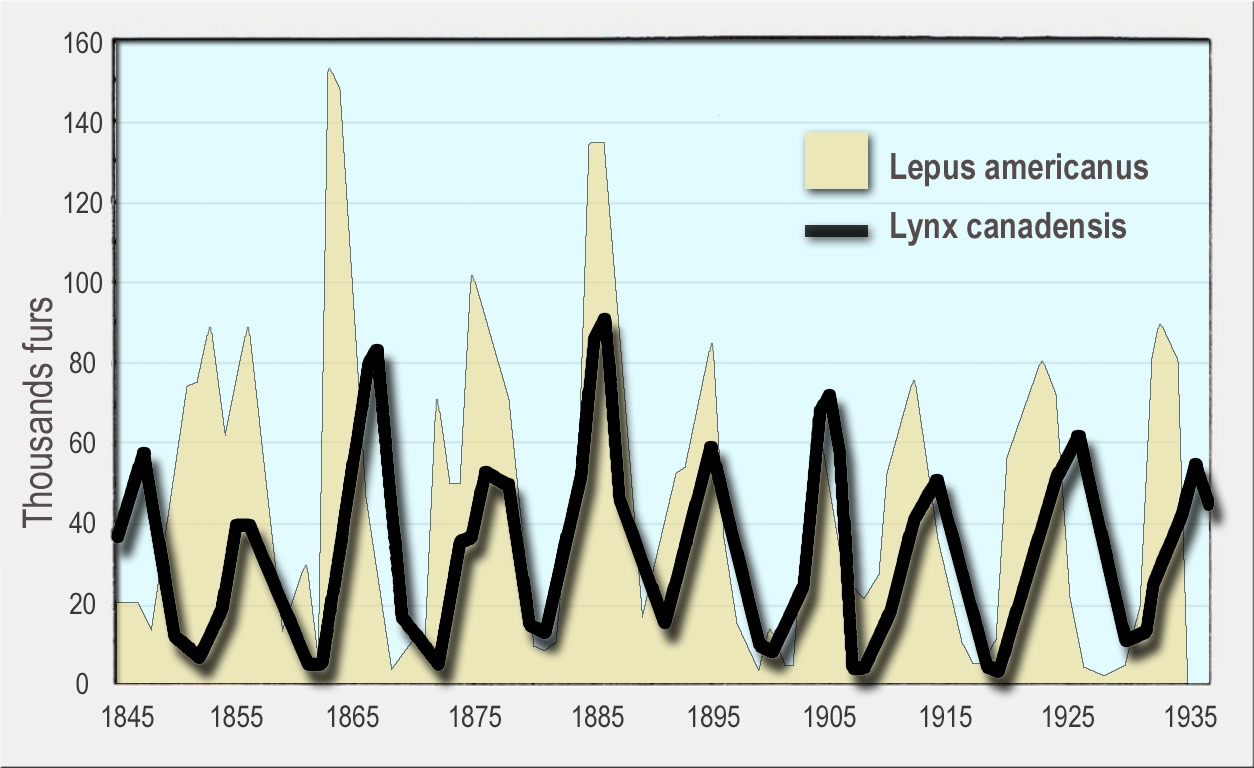
\includegraphics[width=0.6\textwidth]{figs/hares-lynx}
\end{frame}


\begin{frame}[fragile]
\frametitle{like \S3.3 \#11, cont.}

\begin{itemize}
\item \emph{example 3., cont.}  solve numerically:
\begin{align*}
\frac{dx}{dt} &= 0.7 x - 1.3 xy & x(0)=1\\
\frac{dy}{dt} &= xy - y  & y(0)=1
\end{align*}
\end{itemize}

\vspace{-2mm}
\noindent \emph{solution.}
\begin{Verbatim}[fontsize=\small]
>> f = @(t,z) [0.7*z(1)-1.3*z(1)*z(2); z(1)*z(2)-z(2)];
>> [tt,zz] = ode45(f,0:.1:60,[1;1]);
>> plot(tt,zz),  xlabel t
>> legend('prey','predators')
\end{Verbatim}

\bigskip
above uses:

$z_1(t)=x(t)$

$z_2(t)=y(t)$

\vspace{-22mm}
\hfill 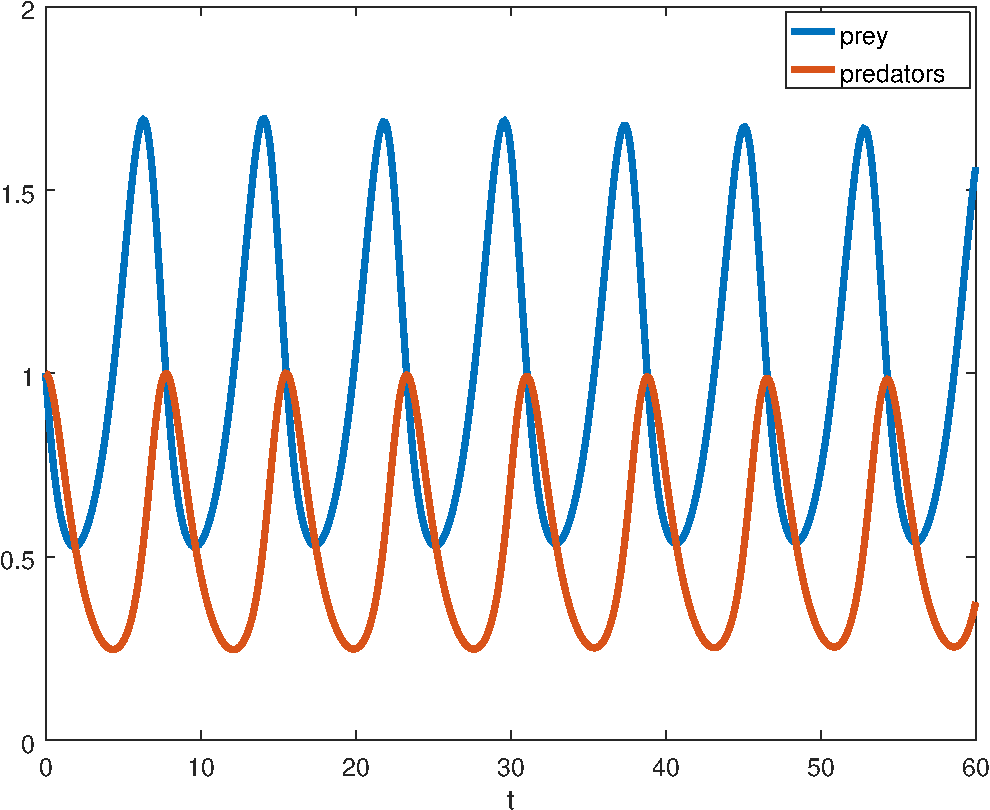
\includegraphics[width=0.45\textwidth]{figs/lotka-time}
\end{frame}


\begin{frame}[fragile]
\frametitle{like \S3.3 \#11, cont.$^2$}

\begin{itemize}
\item a different view is to plot $x=z_1$ versus $y=z_2$
\end{itemize}

\begin{Verbatim}[fontsize=\small]
>> figure(2)
>> plot(zz(:,1),zz(:,2),'k')
>> xlabel('x(t)  prey'),  ylabel('y(t)  predators')
\end{Verbatim}

\bigskip
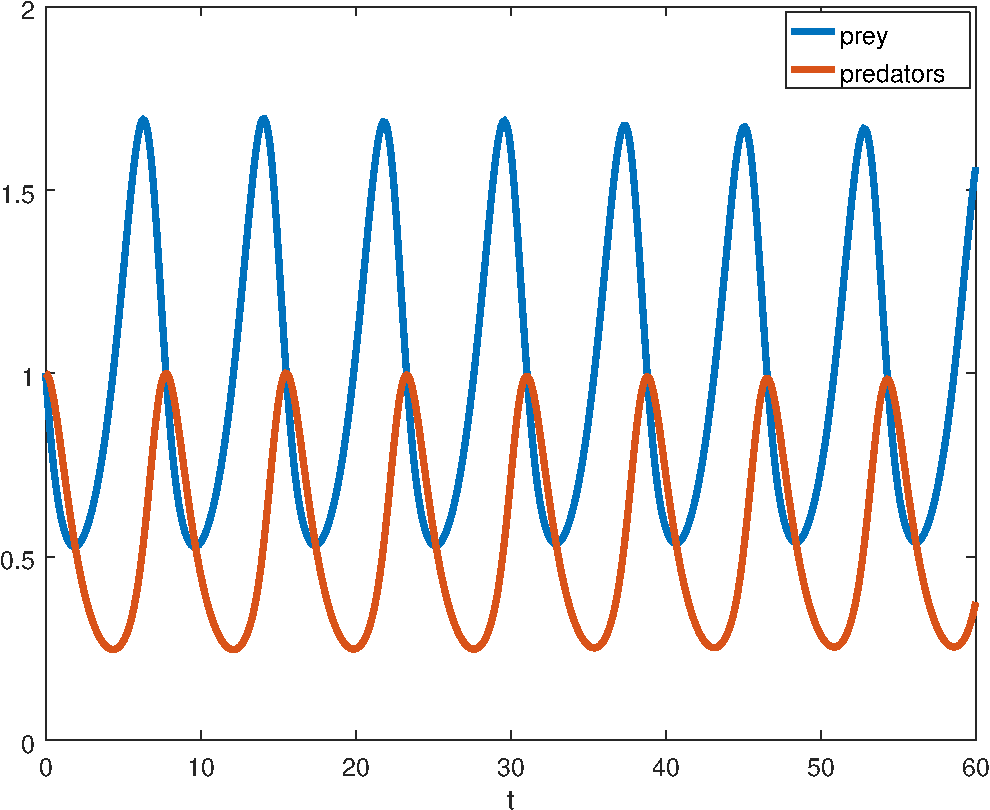
\includegraphics[width=0.44\textwidth]{figs/lotka-time}\quad 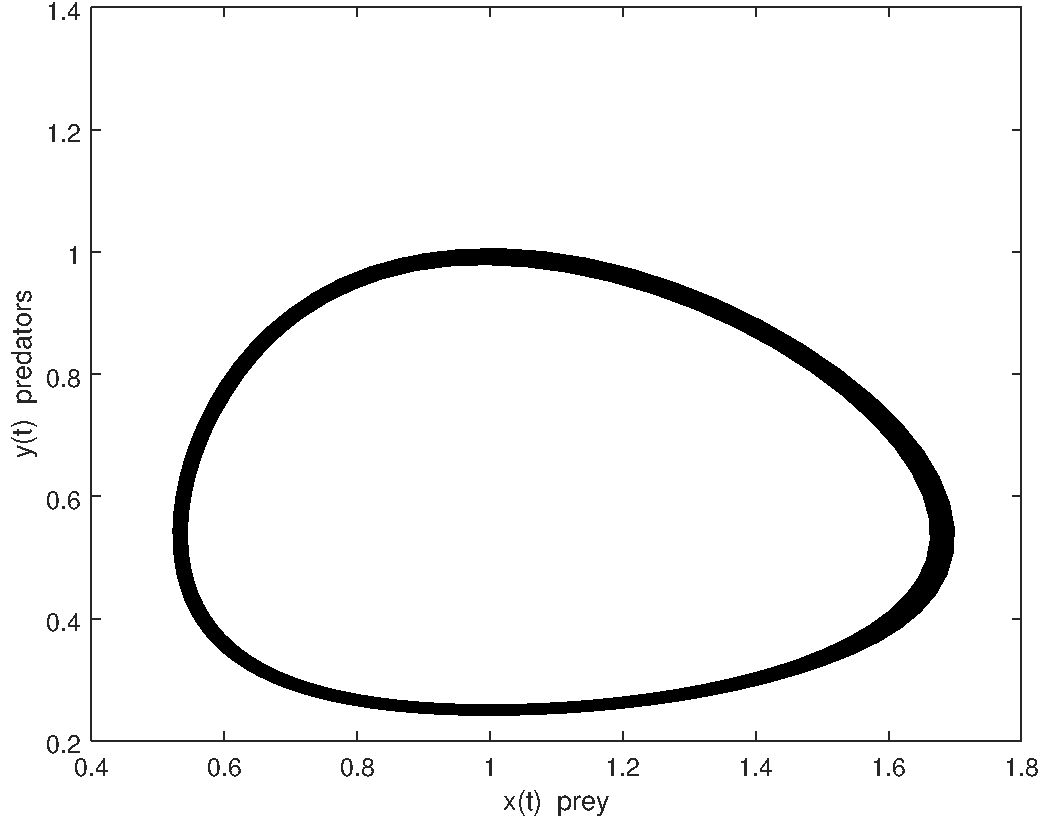
\includegraphics[width=0.46\textwidth]{figs/lotka-phase}
\end{frame}


\begin{frame}{beyond: PDEs and pattern generation}

\small
\begin{itemize}
\item consider this system of ODEs ($\phi,\kappa$ constants):
\scriptsize
\begin{align*}
\frac{du}{dt} &= -uv^2+\phi(1-u) \\
\frac{dv}{dt} &= uv^2-(\phi+\kappa)v
\end{align*}
\small
\item a model for chemical reactions\footnote{\tiny J.~E.~Pearson (1993). \emph{Complex patterns in a simple system}, Science, 261, 189--192} with two chemicals $u$ and $v$, similar to a predator-prey system
\item add diffusion:

\vspace{-10mm}
\scriptsize
\begin{align*}
\frac{\partial u}{\partial t} &= D_u \left(\frac{\partial^2 u}{\partial x^2} + \frac{\partial^2 u}{\partial y^2}\right) -uv^2+\phi(1-u) \\
\frac{\partial v}{\partial t} &= D_v \left(\frac{\partial^2 v}{\partial x^2} + \frac{\partial^2 v}{\partial y^2}\right) + uv^2-(\phi+\kappa)v
\end{align*}
\small
% in biology the way you get many patterns (e.g.~spots on a cheetah) is to have a competition between two chemicals at every location; each location has a first-order ODE system going, and they are linked together by diffusion
\end{itemize}

\mbox{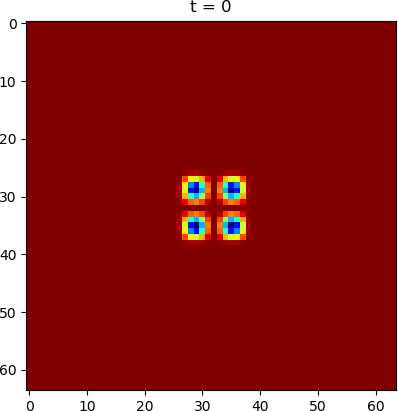
\includegraphics[width=0.23\textwidth]{figs/pattern0}\quad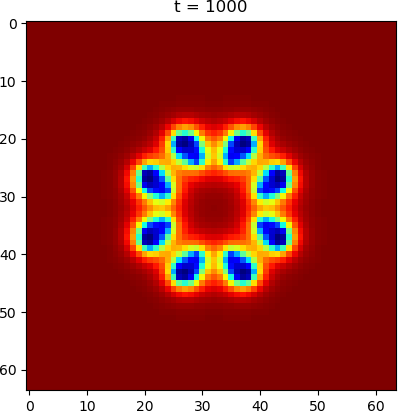
\includegraphics[width=0.23\textwidth]{figs/pattern2}\quad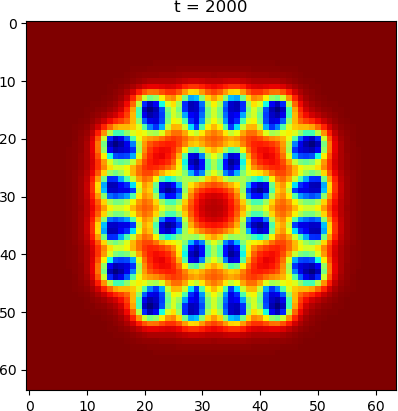
\includegraphics[width=0.23\textwidth]{figs/pattern4}\quad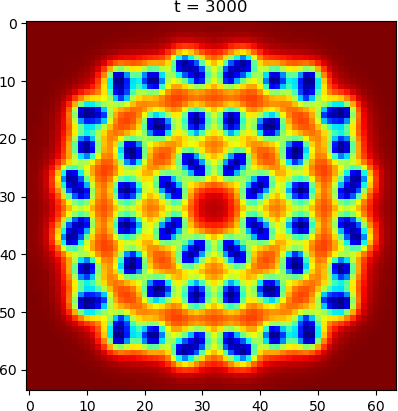
\includegraphics[width=0.23\textwidth]{figs/pattern6}}

\bigskip
\end{frame}


\begin{frame}{expectations}

\begin{itemize}
\item just watching this video is \emph{not} enough!
     \begin{itemize}
     \item see ``found online'' videos and stuff at

     \centerline{\href{https://bueler.github.io/math302/week13.html}{\tt \color{cyan} bueler.github.io/math302/week13.html}}
     \item \emph{read} \S3.3
     \item \emph{do} the WebAssign exercises for section 3.3
     \end{itemize}
\end{itemize}
\end{frame}

\end{document}

